% C.22 矩形 3x4, 对角线
\documentclass[tikz,border=4pt]{standalone}
\usepackage{ctex}
\usepackage{amsmath}
\usetikzlibrary{calc, arrows.meta}
\begin{document}
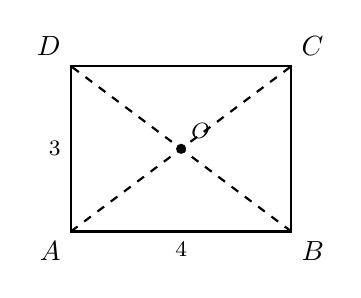
\begin{tikzpicture}[scale=0.7, thick]
  \coordinate (A) at (0,0);
  \coordinate (B) at (4,0);
  \coordinate (C) at (4,3);
  \coordinate (D) at (0,3);
  \coordinate (O) at (2,1.5);
  \draw (A) -- (B) -- (C) -- (D) -- cycle;
  \draw[dashed] (A) -- (C);
  \draw[dashed] (B) -- (D);
  \filldraw (O) circle (2pt);
  \node[below left] at (A) {$A$};
  \node[below right] at (B) {$B$};
  \node[above right] at (C) {$C$};
  \node[above left] at (D) {$D$};
  \node[above right, font=\footnotesize] at (O) {$O$};
  \node[font=\footnotesize, below] at (2,0) {$4$};
  \node[font=\footnotesize, left] at (0,1.5) {$3$};
\end{tikzpicture}
\end{document}
